\section{Fresh confirmation, nonseparable sensing and proposal development}
\label{app:paper-level-results}

\paragraph{Learned-cohort design.}
The development set crosses training seeds $0,1$ with data seeds $800$--$803$. Nine configurations give 72 cells. The selection rule first requires mean W1 within $0.002$ of the joint full-factor baseline, then chooses the fastest eligible anchored setting. It selects $N=8192,K=1024,M=8$ before confirmation. Five fixed checkpoints crossed with data seeds $900$--$919$ give 100 paired targets. Four settings produce 400 confirmation cells. Every reference, source receipt, dataset regeneration and strict checkpoint reload is independently checked. The independent reference uses 131073 integration nodes. Maximum W1 discrepancies are $1.14\times10^{-6}$ for the learned target and $1.06\times10^{-6}$ for the true target.

The fixed two-way paired bootstrap has 10000 replicates and seed 20260930. The primary gate requires both one-sided 95\% upper bounds: W1 degradation at most $0.002$ and ratio of mean elapsed times below $0.8$. The selected anchor passes against the original joint baseline, with time ratio $0.20341$ and W1 difference $-0.000643$ (two-sided interval $[-0.003037,0.001764]$). It fails against the original coordinatewise baseline, with W1 difference $0.003523$ (interval $[0.001565,0.005545]$). The original-budget anchor $N=32768,K=2048,M=4$ has W1 $0.01988$ in $3.864$ seconds. Time includes method-specific preparation and sample return, but excludes shared references and one-time density-network prediction. These networks do not evaluate neural scores at every diffusion step.

\paragraph{Equal-budget ablation.}
This comparison was added after the original confirmation results were visible. It is explicitly post-hoc. On the same 100 targets, all methods use $N=8192,K=1024$ with the original paired seeds and randomized execution order (seed 20261003). The 100 anchored replays agree with their original saved particles and weights to the recorded numerical tolerance. The two additional baselines and replays give 300 cells, all recovered and independently audited. Sources and raw receipts are checked, all five checkpoints are reloaded, and the same-target reference integrals and same-grid population certificates are reused from the passed parent audit.

The anchored-to-joint ratio of mean times is $0.87967$ with paired 95\% interval $[0.87047,0.89000]$. Its W1 difference is $-0.001681$, interval $[-0.005470,0.001359]$, with one-sided upper bound $0.000924$. Against coordinatewise weighting, the time ratio is $0.82492$, interval $[0.81458,0.83785]$, while the W1 difference is $0.002407$, interval $[0.000250,0.004574]$. Neither comparison passes the inherited joint diagnostic requiring time ratio below $0.8$ and W1 degradation at most $0.002$. The latter reference also violates the accuracy allowance. Figure~\ref{fig:paper-level-diagnostics} separates configuration effects from method effects.

\begin{figure}[h]
\centering
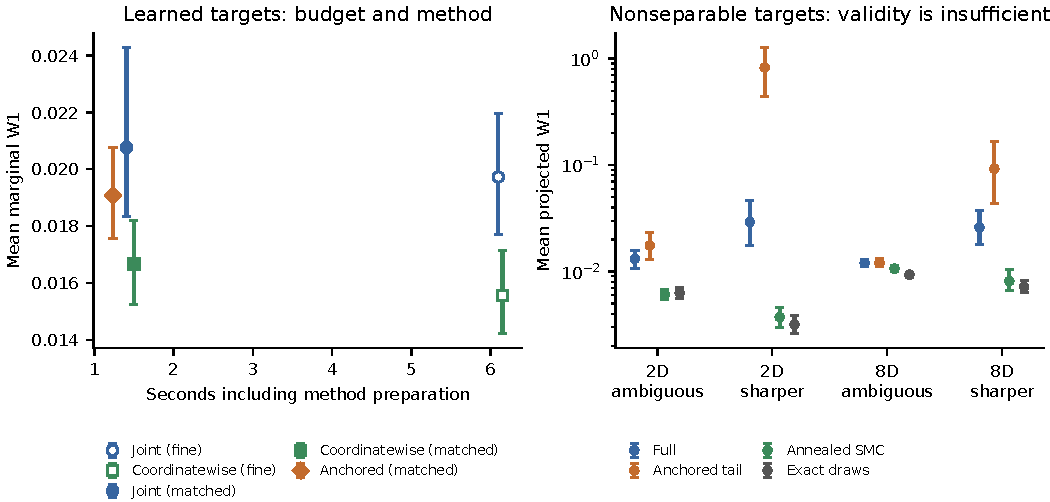
\includegraphics[width=\linewidth]{figures/paper_level_diagnostics.pdf}
\caption{Left: changing the particle/grid budget accounts for most of the original elapsed-time gap. Filled markers use the matched budget; error bars are two-way bootstrap 95\% W1 intervals on the same 100 targets. Right: full and tail-controlled methods share strict integrability certificates, but their nonseparable finite-particle errors differ substantially. Error bars use twenty shared seed clusters.}
\label{fig:paper-level-diagnostics}
\end{figure}

\paragraph{Sensor generator and exact reference.}
Each sensor direction is normalized from a seeded Gaussian vector. In the regular regime, its first two coordinates are replaced by cosine/sine directions on perturbed angles before normalization. Component prior probabilities alternate between $0.65$ and $0.8$. Noise standard deviations lie in $[0.8,0.95]$ for the ambiguous regime and $[0.35,0.43]$ for the regular regime. The latter label denotes sharper observations; sign ambiguity remains. Given one observation, component means are $\pm y_ga_g/(\sigma_g^2+\|a_g\|^2)$ and covariance is $I-a_ga_g^\top/(\sigma_g^2+\|a_g\|^2)$. Enumeration of all signs yields an exact Gaussian mixture, with a common component covariance and exact mixture moments. The independent auditor also computes evidence in observation space and compares the resulting direct likelihood density with this latent-space mixture.

Development seeds $1100,1101$ crossed with both dimensions and regimes yield eight targets and 96 cells. Anchored control fails its development accuracy screen; the predefined least-error fallback selects $N=16384,K=2048,M=8$, with the failure flag retained. The likelihood baseline selects 64 annealing stages, three pCN moves per stage with scale $0.15$, and one global sign-flip Metropolis move. Confirmation seeds $1200$--$1219$ give 80 targets and six methods, for 480 cells. The bootstrap resamples the same data-seed index across dimensions, regimes and methods, for 10000 replicates with seed 20261001.

\begin{table}[h]
\centering\small
\caption{Mean projected W1 by nonseparable setting; twenty seeds in each column.}
\begin{tabular}{lrrrr}
\toprule
Method & $d=2$, ambiguous & $d=2$, regular & $d=8$, ambiguous & $d=8$, regular\\
\midrule
Full & 0.01318 & 0.02917 & 0.01207 & 0.02603\\
Raw batch & 0.01192 & 0.05998 & 0.01236 & 0.02882\\
Fixed tail & 0.02257 & 1.02687 & 0.01409 & 0.51651\\
Anchored tail & 0.01757 & 0.82317 & 0.01203 & 0.09216\\
Annealed SMC & 0.00612 & 0.00373 & 0.01064 & 0.00811\\
Exact draws & 0.00631 & 0.00317 & 0.00934 & 0.00717\\
\bottomrule
\end{tabular}
\end{table}

The independent sensor audit covers all 88 reference assets and all 576 development/confirmation cells. It checks raw sample metrics, exact density and moment calculations, matrix certificates, checksums, configurations and completion markers. Seeded reference samples are reproduced in their original numerical environment. Cross-platform singular-value decompositions can rotate or change signs of Gaussian sampling factors; the local cross-platform report retains the resulting samplewise replay mismatches while all independently recomputed posterior densities, moments and cell metrics agree. Timing is excluded from confirmatory inference because an unrelated training process overlapped the final sampling interval. Raw-batch full-history matrix integrability remains explicitly unclassified.

\paragraph{Gaussian path pilot.}
New seeds $1300,1301$ crossed with both sensor dimensions and regimes give eight development targets. Seven configurations give 56 cells. The proposal uses exact Gaussian backward recursion, independent paths without intermediate resampling, and full path likelihood-ratio correction; a two-component variant uses the complete mixture-density denominator. All full-target proposals share the same specified full Euler target at a given grid. The batch-eight variant targets its own random kernel. Source code, exact references, all final metrics and log-weight normalization are independently audited. Eleven implementation tests pass on the H20, including dense-path Gaussian agreement and nonlinear complete-path density identities.

\begin{table}[h]
\centering\small
\caption{Gaussian path development only. The stopping rule admits no candidate for confirmation. Different particle/grid budgets are shown explicitly.}
\begin{tabular}{lrrrr}
\toprule
Proposal/target & $N$ & $K$ & Projected W1 & Seconds\\
\midrule
Mean Gaussian/full & 8192 & 1024 & 0.22192 & 1.051\\
Anchor Gaussian/full & 8192 & 1024 & 0.26545 & 1.047\\
Two Gaussians/full & 8192 & 1024 & 0.12567 & 1.182\\
Two Gaussians/full & 16384 & 2048 & 0.14606 & 3.012\\
Two Gaussians/batch-eight & 8192 & 1024 & 0.34275 & 1.567\\
Original full weighting & 16384 & 2048 & 0.02500 & 1.633\\
Annealed SMC & 16384 & 64 stages & 0.00702 & 0.106\\
\bottomrule
\end{tabular}
\end{table}
